\section{Evaluation}
\label{sec:evaluation}

In this section, we evaluate the performance of our MapReduce framework using several test cases. We first describe the experimental setup and datasets in Section~\ref{subsec:experimental-setup} and Section~\ref{subsec:datasets}, respectively. We then present the results of the WordCount application in Section~\ref{subsec:word}. Finally, we evaluate the performance of our framework under different parameters in Section~\ref{subsec:para}. 

\subsection{Experimental Setup}
\label{subsec:experimental-setup}

In this part, we describe the experimental setup used to evaluate the performance of the implemented MapReduce framework. We run the framework on a single machine with multiple threads. It is equipped with an Intel Core i7-12700H CPU, 32 GB of RAM, and a 2 TB SSD. The software environment ran on Ubuntu 22.04 LTS in Windows Subsystem for Linux (WSL) 2.0., with Java being the primary programming language. We use JDK 21 for compiling and running the code, gRPC 1.68.0 for communication between the master and worker nodes, and JUnit 4.13.2 for testing. For each experiment, we perform 3 runs and adopt the Pareto principle to select the optimal result. For the cluster setup, we use Docker containers to simulate the distributed environment. The docker version is 26.1.1.

\begin{table}[!t]
    \centering
    \caption{Datasets used for evaluation.}
    \label{tab:datasets}
    \begin{tabular}{c c c}
        \hline
        \textbf{Dataset} & \textbf{Words} & \textbf{Size (KB)} \\
        \hline
        A Christmas Carol & 29,282 & 164 \\
        King Solomon's Mines & 82,197 & 444 \\
        Oliver Twist & 157,967 & 880 \\
        Random Words\textsuperscript{\dag} & 13,848,900 & 102,404 \\
        \hline
    \end{tabular}
    \vspace{0.5em} \\
    \footnotesize{\textsuperscript{\dag} A randomly generated dataset by a Python script.}
\end{table}

\subsection{Datasets}
\label{subsec:datasets}

We use four datasets for the evaluation of our MapReduce framework, as shown in Table~\ref{tab:datasets}. The first three datasets are classic novels, including \textit{A Christmas Carol}, \textit{King Solomon's Mines}, and \textit{Oliver Twist}. The fourth dataset is a random dataset with a size of 100 MB, which is generated by a Python script.

\begin{table}[!t]
    \centering
    \caption{Performance of the WordCount application using our MapReduce implementation.}
    \label{tab:wordcount}
    \begin{tabular}{|c|c|c|}
        \hline
        \textbf{Dataset} & \textbf{Time (s)} \\
        \hline
        A Christmas Carol & 0.625 \\
        King Solomon's Mines & 0.759 \\
        Oliver Twist & 0.946 \\
        Random Words & 5.84 \\
        \hline
    \end{tabular}
\end{table}

\subsection{Word Count Application}
\label{subsec:word}

In this part, we present the results of the WordCount application using our MapReduce framework. As shown in Table~\ref{tab:wordcount}, we measure the execution time of the WordCount application using different datasets. We can see that the time increases with the size of the dataset, which is expected due to the increased number of words to process. For the classic novels, our implementation process the data in less than $1$ second, showcasing the high efficiency of our framework. For the random dataset, the execution time is significantly higher than the classic novels, as it contains more words. Overall, the results demonstrate that our framework can efficiently process large datasets and generate the word count in a short time.

\begin{figure}
    \centering
    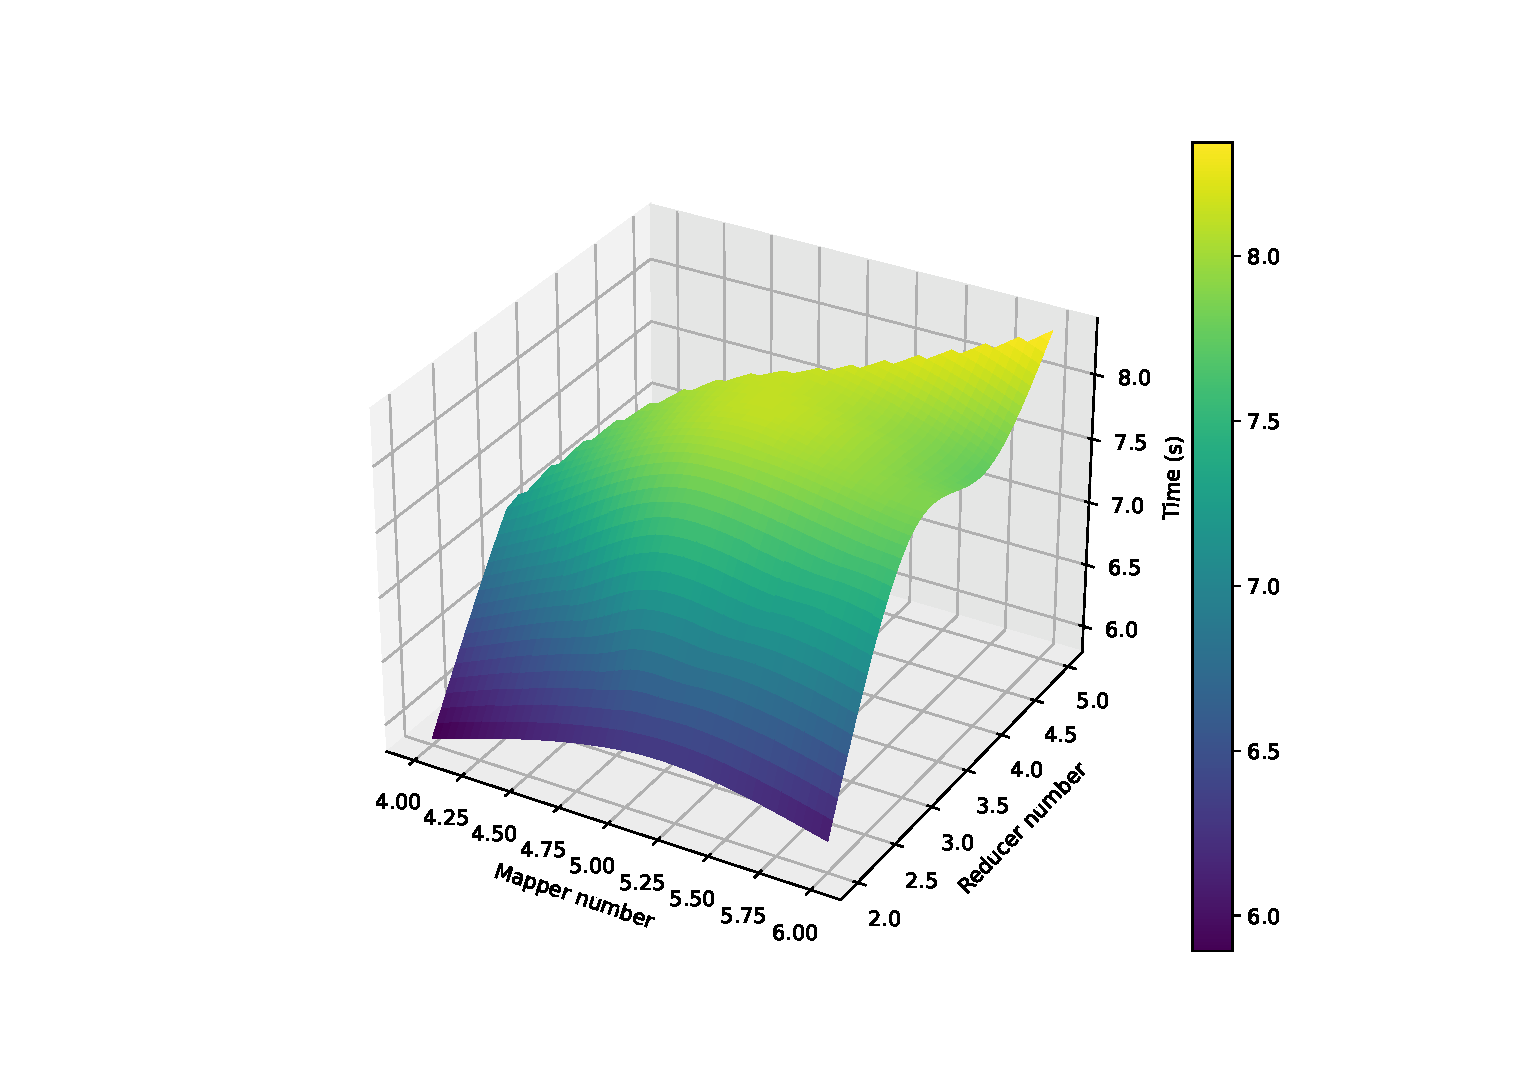
\includegraphics[width=0.5\textwidth]{num}
    \caption{Performance of the WordCount application using different numbers of worker nodes.}
    \label{fig:wordcount}
\end{figure}

\subsection{Parameter Variation}
\label{subsec:para}

In this part, we evaluate the performance of our MapReduce framework under different parameters, i.e., the number of the Mappers and the number of the Reducers. We use the \textit{Random Words} dataset for this experiment. As shown in Figure~\ref{fig:wordcount}, we measure the execution time of the WordCount application using different numbers of worker nodes. We can see that the execution time decreases as the number of worker nodes increases, which is expected due to the increased parallelism in processing the data. However, the performance improvement diminishes as the number of Reducers increases. This can be explained that the overhead of gRPC communication between the master and worker nodes increases with the number of Reducers. Overall, the results demonstrate that our framework can efficiently scale across multiple nodes and optimize the performance of the job.